\chapter{Characteristics of Open Street Map}
	
\section{General}
The OpenStreetMap is one of the most impressive projects of Volunteered Geographic Information on the Internet\cite{Neis2012}. Until recent the mapping of the Earth was preserved highly skilled, well-equipped and organized individuals and groups. One important happening was in 2000 when Bill Clinton removed the selective availability of the GPS signal \ref{sec:weber}. This change improved the accuracy of simpler, cheaper GPS receivers so that also ordinary people could start mapping their movements. OpenStreetMap was founded in 2004 at University College London by Steve Coast. The goal was to create a free database with geographic information of the world \cite{Neis2012}. Back in 2004 the geographic data was expensive and hard to get access to. 

The OSM project stands out from other data sources mainly because its free to use and its released under a license that allows for pretty much whatever the user wants to as long as the user mention the original creator and the licence\cite{Chilton}.  The most common contribution approach is to record data using a GPS receiver and edit the data using one of the free and available OSM editors \cite{Neis2012}.  

One of the reasons to OpenStreetMap's success is that today the world has a need for instant information, particularly in crisis situations \cite{Chilton}. Here OpenStreetMap is the leading global example of the effictiveness of crowdsourcing of geodata. Crowdsourced geographic data has characteristics or advantages of large data volume, high currency, large quantity of information and low cost \cite{Wang2013}. The project are changing the way individuals and organisations are thinking about the collection process, purchase and use of geodata \cite{Chilton}.  

%\section{Culture}
%OSMhas no notability rule, an arbitrary amount of detail is possible, but somebody has to maintain it! %https://www.youtube.com/watch?v=KNTSZGnQVRw

\section{Data structure}
OpenStreetMap uses a topological data structure. This sturcture includes three basic components nodes, ways and relations. Nodes are points with a geographic position stored as coordinates (Lat, long) according to WGS84. Ways are lists of two or more nodes, representing an open- or closed way, used to describe streets, rivers, among others \cite{Debruyne2015}. A relation is a multi-purpose data structure that documents a relation between two or more components \cite{OpenStreetMapg}. OpenStreetMap's structure uses tags to add metadata to geographic objects. Tags consist of two items, a key and a value of the form key=value. The key is used to describe the topic, category or type of feature, while the value describes the details of the specific form of the key specified. A example of a key-value pair can be building=church, here the key is building and the value is church, this is a building that was built as a church. 

OpenStreetMap do not have any restrictions on tags assigned to nodes, ways or relations, mappers can use any key-value pair in their import. Nevertheless, the norm in OSM is to try to map new data with existing tags. Good practice is to search for tags, or Map Features, on different OSM wiki-sites. On the \textit{tags you like} wikipage they recommend different sites, but points out \textit{taginfo.openstreetmap.org} as the most useful site. Taginfo is a website created for finding and aggregating information about OSM tags, it covers the whole planet and is updated daily. The web page list tags used in the database and also inform on how often they have been used.* %How frequent they appear insted?
 Taginfo also lists other tags which have been used in combination with the tags you searched for. Some countries also have their own taginfo web pages, like Ireland, Great-Britain and France, Norway do not have their own taginfo web page. If a mapper doesn't find an appropriate key-value pair and want to create a new feature this has to be documented on the OSM wiki page. 
 
%Verifiability: From a given scenario, a tag/value combination is verifiable if and only if independent users when observing the same feature would make the same observation every time.\href{http://wiki.openstreetmap.org/wiki/Verifiability}. 

A changeset in OpenStreetMap is a collection of changes made by one user over a short period of time \cite{OpenStreetMapi}.  A change can be creation of new components, adding of tags to existing components, changes to tags in existing components, removal of tags and removal of components. Changes are added to the changeset as long as it's open, changesets are either closed directly or by itself after a period of inactivity (currently one hour). Every component in the OSM database is a part of a changeset.* %Hvert element i OSM databasen er en del av et changeset, skrive om?

\section{Organization}
%Redgjøre for hva OSM er og hvordan det fungerer teknisk og organisatorisk
The OpenStreetMap Project is supported by the OpenStreeMap Foundation (OSMF) which is a UK-registered non-profit organization. The foundation was founded in 2006 and consists of members from all over the world, as of December 2015 consist of 350 normal-, 351 associate- and 18 corporate members \cite{OSMF2015}. OSMF include a board of seven members and is critical to the ongoing function and growth of the OpenStreetMap project \cite{OSMF}.  The foundation has the responsibility for the servers and services necessary for hosting the OSM project. They also support and communicates with the working groups, and delegates tasks that has to be done, like web site development etc. 

A person can contribute to the OSM project without being a member of the foundation. The project has over 3 million registered users \cite{OSMProject2016} who are collecting, updating and editing the data. The crowdsourced data are then released under the Open Database License, \textit{"a license agreement intended to allow users to freely share, modify, and use this Database while maintaining this same freedom for others"} \cite{ODbL}.  Users can edit maps through different tools made by OSM developers. One tool is called iD and is the default web browser editor written by MapBox. There are also desktop editing applications like JOSM and Merkaartor which are more powerful and better suited for advanced users. 

Communication is done through channels like mailing lists, wiki-pages, conferences and Github repositories. In the public mailing lists everyone who subscribes to it is overhearing every conversation. This is described as broadcast communication in the Gutwin paper from 2004 \cite{Gutwin2004}. The ability to speak to an expected audience rather than one individual has several advantages. Allowing people to decide for themselves whether to respond or not and as the conversation develops new people can join. In OpenStreetMap there are over 150 mailing lists \cite{Reiter2016}, keeping an overview of everything is impossible. That is why weeklyOSM was created in 2010 and is a collection of news relevant for the OSM community written in 5 different languages \cite{Freyfogle2016}.  In State of the Map 2016 conference the WeeklyOSM team won the Influential Writing Award, nominated and voted by the community [OpenStreetMap, 2016a]. A good evidence of how important their work is for the community. State of the map is the main OSM conference, organized by OSMF and has been held each year since 2007 \cite{OpenStreetMapj}. Important communication is also done through both issues and pull requests in the repositories at the OpenStreetMap Github channel. 

%The degree to how to get involved in OSM is depp.  mapping, software processes etc., this keeps people interested. One problem is the communication through the different groups, the energy level is not high enough.  Lots of people exited about communication, everyone have a obligation to show they use their different possibilities \cite{Maron2016}.   

%Mer om OSM Foundation Success & Scale in a Data-Producing Organization s 4119, Org&ikt mappen

 \section{File format, .osm files}
The .osm file format is specific to OpenStreetMap and it is not easy to open these files using GIS-software like QGIS. The file format is designed to be easily sent and received across the internet in a standard format. Therefore .osm files are easily obtained, but using the files directly to do analysing and map design is not easy. The .osm files are coded in the XML format. It is recommended to convert the data into other formats when using the files \href{http://learnosm.org/en/osm-data/file-formats/}{source}. 

Points are represented as nodes, lines as ways and areas as relation in .osm files. Each represented by a tag: <node>, <way> and <relation>. Node is one of the core elements in the OSM data model. A node-tag consists of a single point defined by node-id, latitude and longitude. When nodes are used on their own they represents point features, normally includes at least one tag to define the points purpose \cite{OpenStreetMapc}. In figure \ref{fig:nodetag} the node tag represents a bag shop named Citybag, a point of interest, where k is key and v is value. User is the name of who last modified the node and uid is the persons numeric user id.  

\begin{figure}[H]
    \centering
    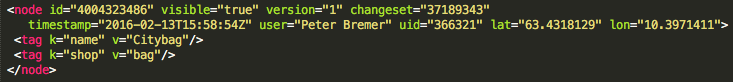
\includegraphics[scale=0.6]{figures/FixedByMe/node_tag.png}
    \caption{Example of a node tag}
    \label{fig:nodetag}
\end{figure} 

A way consists of two or more nodes and can either be open or closed. An open way describes a line feature not sharing first and last node. Features can be roads, cycleway, streams etc.* %Kan man skrive etc paa engelsk?
When a way is closed the first and last nodes are the same and can be interpreted as a closed polyline or an area, or both \cite{OpenStreetMapd}. A closed way with highway=* tag can represent roundabouts, and if it has amenity=school tag the closed way can represent the outline of a school. In figure \ref{fig:waytag} the way represents a building since k=building and v=yes. The buildings address is also added and its name. The <nd> tag represents a node, where all the <nd> tags creates the building footprint. Note that the first and last <nd> tag refers to the same node. 

\begin{figure}[H]
    \centering
    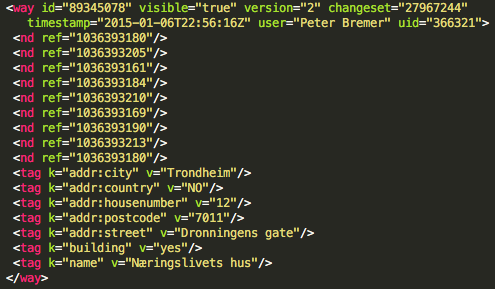
\includegraphics[scale=0.7]{figures/FixedByMe/way_tag.png}
    \caption{Example of a way tag}
    \label{fig:waytag}
\end{figure} 

A relation is an ordered list of one or more nodes, ways and/or relations and is used to define logical or geographical relationships between the other elements  \cite{OpenStreetMape}. If a building consists of multiple parts, tagged with building:part=*, a relation is used to define the geographical relationship between the parts. It is possible to specify roles to different parts, a road can have role as east, going towards east. In multi polygons parts can have an inner or outer role, to specify whether it forms the inner or outer part of the polygon. A building relation is shown in figure \ref{fig:reltag}. There are two members in this relation, both are ways, first has an outer role and the second has an inner role in the multi polygon.  

\begin{figure}[H]
    \centering
    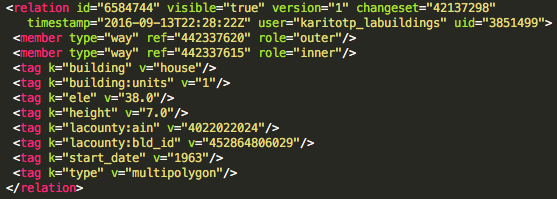
\includegraphics[scale=0.7]{figures/FixedByMe/relation_tag.png}
    \caption{Example of a relation tag}
    \label{fig:reltag}
\end{figure} 

 \section{Mapping buildings in OSM}
When importing buildings into OSM the building the relation representing it must be tagged Building=*. The building key is used to mark areas as buildings, the * value varies. Frequent occuring values are house, residential and garage, describing the buildings specific usage. The most frequent occurring value to the building key is yes and used when its not possible to determine a more specific value \cite{OpenStreetMapf}. A list of possible values that can be added to the building key is listed on the OSM building wiki page. It is possible to introduce new values, but it is not recommended. Additional attributes often used together with the building key is entrance, height of the building, building levels, address and so on. The building key is most common used in way representations. For an example of how to use building key in a way-tag see figure \ref{fig:waytag}.

A building can be represented by nodes, ways or relations. Using the building tag on nodes is tolerated but not recommended. A building is much better represented with their footprint (close way or multi polygon), if the footprint is available one should not add building tag in nodes. It is most common to represent buildings through ways \cite{OpenStreetMapf}. A building can also be represented with a relation. Relation is used if the building consists of multiple parts which physical differ from each other, often when a 3D representation of the building is created. A building relation mainly consist of two or more way's. A way then represents a part of the building and should be tagged with a building:part key and usually the value yes. Then the ways representing the different building parts are ordered together inside the relation. The relation is then tagged with the key building and a value. See figure \ref{fig:relationtag} for a building representation in a relation. If the relation is tagged with type=building it groups both building footprint and all building parts together. 
